\documentclass[11pt]{article}
\usepackage{graphicx}

\begin{document}

\begin{figure}

\begin{center}

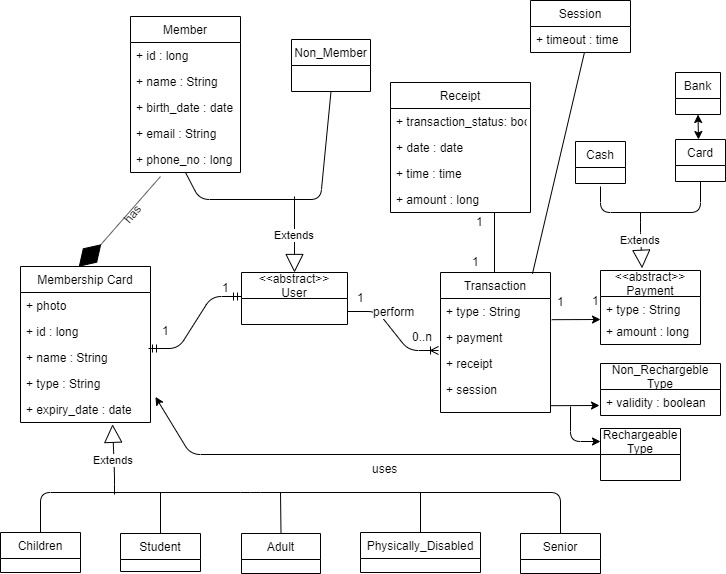
\includegraphics[scale=0.6]{./DomainModel}

\end{center}

\end{figure}

The problem domain of IGo system is represented by a set of concepts, properties and their relationships to each other. The concepts have been modelled as classes and their attributes represent the properties. The classes are also connected to each other and the connections have been labelled wherever relevant.

The central component of the IGo domain is the User class which has been made abstract as the user has to be a member or non-member of the STM service and cannot have an existence otherwise. Member user has attributes recorded as it will be used for the membership card that he/she owns. The Membership Card class further is extended by 5 subclasses which depict the different types of cards allotted to users on the basis of age and other factors. Attributes of non-member user class are not relevant as he/she will be performing onetime transaction that does not make use of any registered passes.

The users interaction with IGo is represented as a Transaction  class which can be of two types : Non Rechargeable or Rechargeable purchase of ticket. If the user is performing a rechargeable transaction, they use the membership card they possess. In either case, payment will be made which is represented by the Payment class. The payment class is abstract as it should be either done through Card or Cash and do not have an independent existence otherwise. If using Card class, then authentication will be done thorough the Bank. Cash payments do not need authentication.

Every transaction provides a receipt indicating the date, time and status of transaction performed and the amount paid, which is represented by the Receipt class. Every transaction also creates a session as depicted by Session class which would expire after the time allotted, after which the transaction will be cancelled.

\end{document}